\section{Durchführung}
\label{sec:Durchführung}
Ziel des Experiments ist es, die Wärmeleitung exemplarisch an Aluminium, Messing und Edelstahl zu untersuchen. 
\subsection{Versuchsaufbau}
%\begin{figure}
%    \centering
%    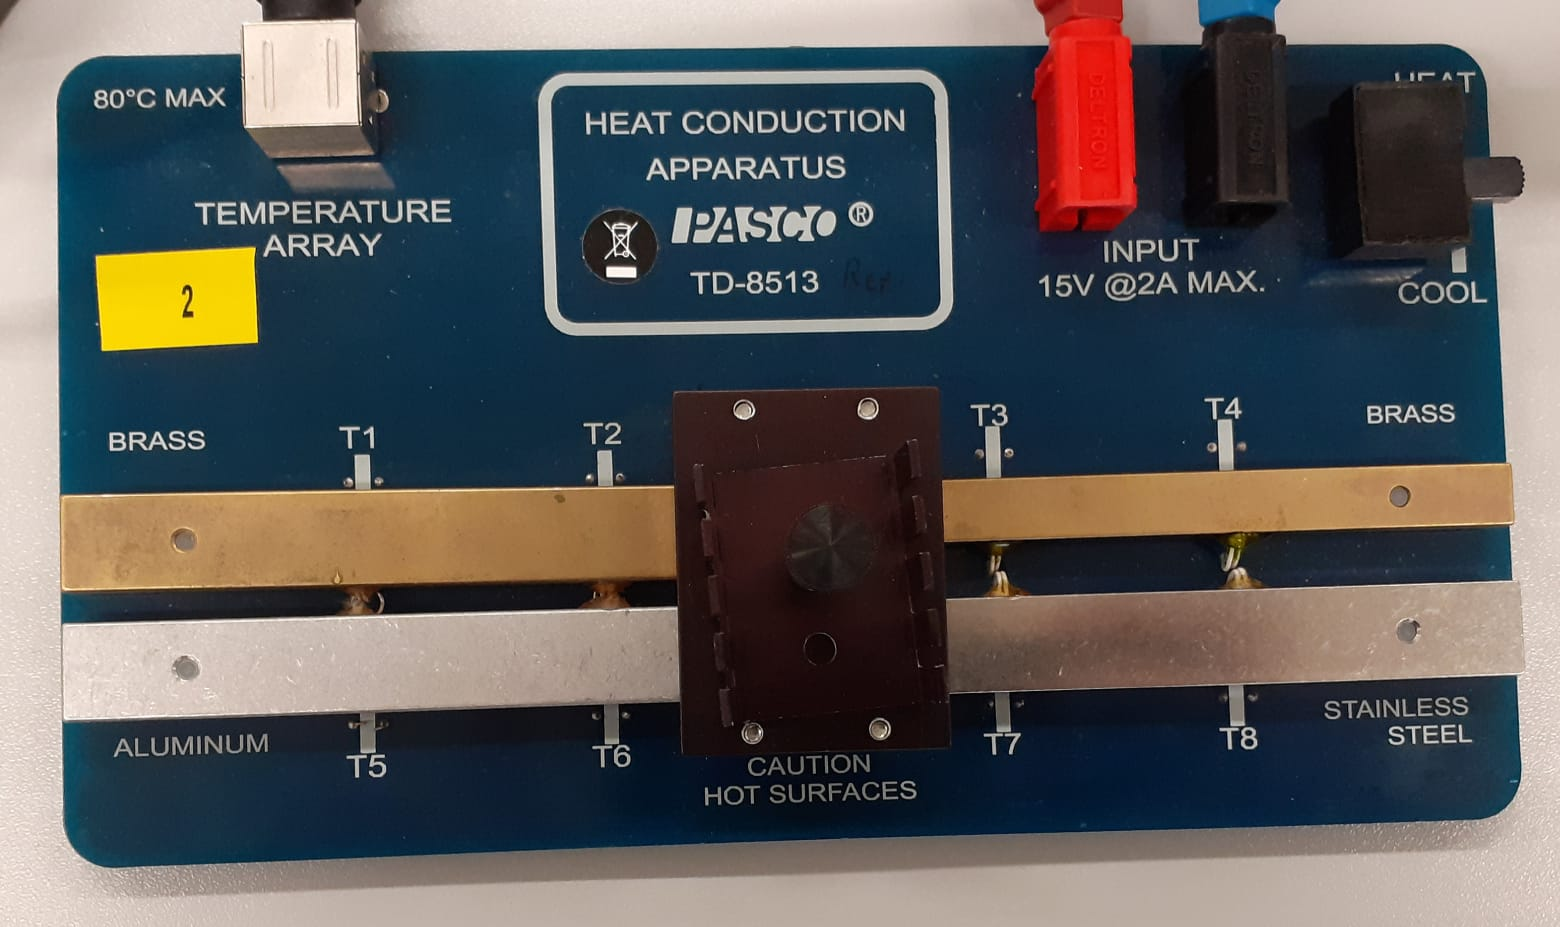
\includegraphics[width=\textwidth]{platine_photo.jpg}
%    \caption{Die zu verwendene Platine.}
%    \label{fig:platine}
%\end{figure}
Auf einer Messplatine sind die verschiedenen Metallstäbe befestigt: 
Jeweils ein Aluminium- und ein Edelstahlstab und zwei Messingstäbe, die sich allein durch ihre Querschnittsfläche unterscheiden.
Es gibt acht Temperaturmessstellen, je zwei pro Stab, die sich in einem Abstand von $\SI{3}{\centi\meter}$ voneinander befinden. 
Je ein Ende wird durch das mittig platzierte Peltier-Element erwärmt oder gekühlt. 
Die Platine wird über ein Temperatur-Array mit dem Xplorer GLX verbunden. 
Das Temperatur-Array ist dafür da, die jeweiligen Temperatursensoren zu identifizieren, sodass die gemessenen Werte den richtigen Sensoren zugeordnet werden.
Die Messwerte werden über den Xplorer GLX, der mit dem Temperatur-Array verbunden ist, aufgenommen und gespeichert. 
Das Peltier-Element wird durch eine Spannungsquelle betrieben, bei der die Spannung reguliert werden kann. 
Eine Wärmeisolierung sorgt dafür, dass der Wärmeaustausch der Metalle mit der Umgebung möglichst gering bleibt.
Bei jeder Messung soll sie also über die Metallstäbe gelegt werden, wohingegen sie zwischen den Messungen entfernt 
werden kann, um den Abkühlvorgang nicht unnötig zu verlängern. 
\subsection{Durchführung}
Es werden insgesamt drei Messreihen aufgenommen: Die Erste mit der statischen, die beiden Folgenden 
mit der dynamischen Methode.\\
Beim ersten Durchgang soll die Temperatur an den Sensoren in einem Zeitintervall der Größenordnung von $\SI{5}{\second}$
gemessen werden. 
Dies wird an dem Xplorer unter dem Menüpunkt \textit{Sensoren} unter \textit{Abtastrate/Intervall} entsprechend eingestellt.
Vor der Messung empfiehlt es sich, alle auf dem Gerät eventuell gespeicherten Daten zu löschen. 
Die Option dazu lässt sich im Menü unter \textit{Daten} finden und ausführen. 
Um sich die Temperaturen der Sensoren anzeigen zu lassen, muss man ins Unterverzeichnis \textit{Digital} gehen.
Nun wird die Spannung auf $\SI{5}{\volt}$ eingestellt und der Schalter rechts oben auf der Platine 
auf \textit{HEAT} gestellt. 
Gleichzeitig wird der mittige Start-Knopf am Messgerät gedrückt, wodurch die Aufnahme der Messdaten in dem vorher
eingestellten Intervall gestartet wird. 
Nun soll so lange gemessen werden, bis der Sensor T7 eine Temperatur von $\SI{45}{\celsius}$ erreicht. 
Dann wird die Messung beendet, die Wärmeisolierung wird entfernt, der Schalter auf der Platine wird auf \textit{COOL} 
umgelegt und der Xplorer wird durch erneutes Drücken der Starttaste in seiner Aufnahme der Messwerte gestoppt. 
Bevor die dynamische Methode gestartet wird, sollten die Stäbe eine Temperatur von $\SI{30}{\celsius}$  
unterschritten haben. \\
Der Xplorer wird nun auf eine Abtastrate von $\SI{2}{\second}$ eingestellt. 
Die Periodendauer der Heiz- beziehungsweise Kühlperioden soll $\SI{80}{\second}$ betragen. 
Demnach wechselt im Folgenden alle $\SI{40}{\second}$ das Peltierelement zwischen Heizen und Kühlen.
Die Spannung soll auf $\SI{8}{\volt}$ eingestellt und mindestens 10 Perioden sollen durchlaufen werden, bevor die Stäbe 
für die dritte Messung erneut gekühlt werden. \\
Dieselbe Methode wird nun für möglichst viele Perioden der Länge $\SI{200}{\second}$ wiederholt, bis einer der Sensoren 
eine Temperatur von $\SI{80}{\celsius}$ erreicht. 
Im Anschluss daran werden die Stäbe wieder auf eine hinreichend niedrige Temperatur abgekühlt und die Messungen sind beendet.
